\documentclass[../package_tutorial.tex]{subfiles}

\begin{document}

作为一个宽泛目的的编程语言,Python被设计为通过多种方式使用。你可以创建网站或者产业机器人或者你朋友玩游戏,所有都使用相同的核心技术。

由于Python的灵活性,所以所有Python项目第一步要思考的是项目的受众和项目对应的运行环境。在写代码之前思考packing似乎是奇怪的,但是这个过程对于避免以后的头痛有奇效。

这篇概述提供了一个解释Python过多packing选项的宽泛意义决定树。继续阅读来为你的下一个项目选择最好的技术。

\subsection{考虑部署}

packages之所以存在是为了被安装(或者部署)的,所以在你package任何东西之前,你将会思考以下问题的答案:
\begin{itemize}
    \item 你的软件用户是谁?你的软件会被其他开发者用来开发软件、被数据中心的操作人员安装或者会被不怎么知道软件的组安装吗?
    \item 你的软件是准备在服务器上运行还是桌面、移动客户端(手机、平板等等)或者是嵌入在专用机器上?
    \item 你的软件是被个体安装还是被大规模安装?
\end{itemize}
packaging完全就是目标环境和开发经验。上述问题有很多答案,每一个组合情形都有它对应的解决办法。有了这些信息,接下来的概述将会指导你找到最适合你的项目的packaging技术。

\subsection{打包Python库和工具}

你可能听说过PyPI,setup.py和wheel文件。这只是Python生态提供给开发者分发Python代码的一小部分工具,为了了解这些,你可以阅读\href{https://packaging.python.org/guides/distributing-packages-using-setuptools/}{打包和分发项目}。

接下来打包的方法是为在开发设定下的技术受众使用的库和工具准备的。如果你正在寻找为了非技术受众或者产品设定的Python打包方法,跳至打包Python应用。

\subsubsection{Python模块}

只依赖标准库的可重分发、重使用的Python文件。你还需要确保它是为了正确的Python版本写的,并仅仅依赖标准库。

如果想要分享简单脚本和代码段的双方有兼容的Python版本(例如通过电子邮件,StackOverflow或者GitHub gists),这是极好的。甚至有一些完整的库将这提供为一个选项,例如bottle.py和boltons。

然而,这种模式不能扩展至包含多个文件、需要额外的库或者需要特定Python版本的项目,因此有了以下选项。

\subsubsection{Python源码分发}

如果你的代码包含多个Python文件,它通常会被组织为一个目录结构。任何一个包含Python文件的目录可以构成一个\href{https://packaging.python.org/glossary/#term-Import-Package}{导入包}。

由于包包含多个文件,所以分发它们更加困难。许多协议支持每次传输一个文件(上次你点击一个下载多个文件的链接是什么时候?)。它更容易得到不完整的传输并且更难保证分发的代码完整性。

只要你的代码只包含Python代码,并且你知道你的部署环境支持的Python版本,那么你就可以使用Python的原生打包工具来创建一个source Distribution Package,简写为sdist。

Python的sdist是一个包含一个或多个包或模块的压缩档案(实际上是.tar.gz文件)。如果你的代码是纯Python的,并且你只依赖于其他的Python包,你可以在\href{https://docs.python.org/3/distutils/sourcedist.html}{这里}学到更多。

如果你依赖于一些非Python代码,或者非Python包(例如lxml中的libxml2,或者numpy中的BLAS库),你将会需要接下来章节详述的格式,它对于纯Python库也有一些好处。

\subsubsection{Python二进制分发}

Python的许多实际能力来自它可以整合软件生态的能力,特别是用C、C++、Fortran、Rust和其他语言写的库。

不是所有的开发者都有正确的工具或经验来构建用这些编译好的语言写得组件,因此Python创建了Wheel——一种被设计用来运载有编译好文物的库的包格式。实际上,Python的包安装器,pip,一直更喜欢wheel,因为安装更快。所以即便是纯Python包也和wheel工作的更好。

当分发须需要与源分发匹配时,二进制分发是最好的。即使你没有为每一个操作系统上传代码的wheel,通过上传sdist,你使得其他平台的用户可以自己构建包。默认情况下会一起发布sdist和wheel,\textit{除非}你在为一种非常特殊的使用场景——你知道你的接受者只需要某一种,创建文物。

Python和PyPI使得一起上传wheels和sdists很容易。只要按照打包Python项目向导就可以了。

\begin{figure}[h]
    \centering
    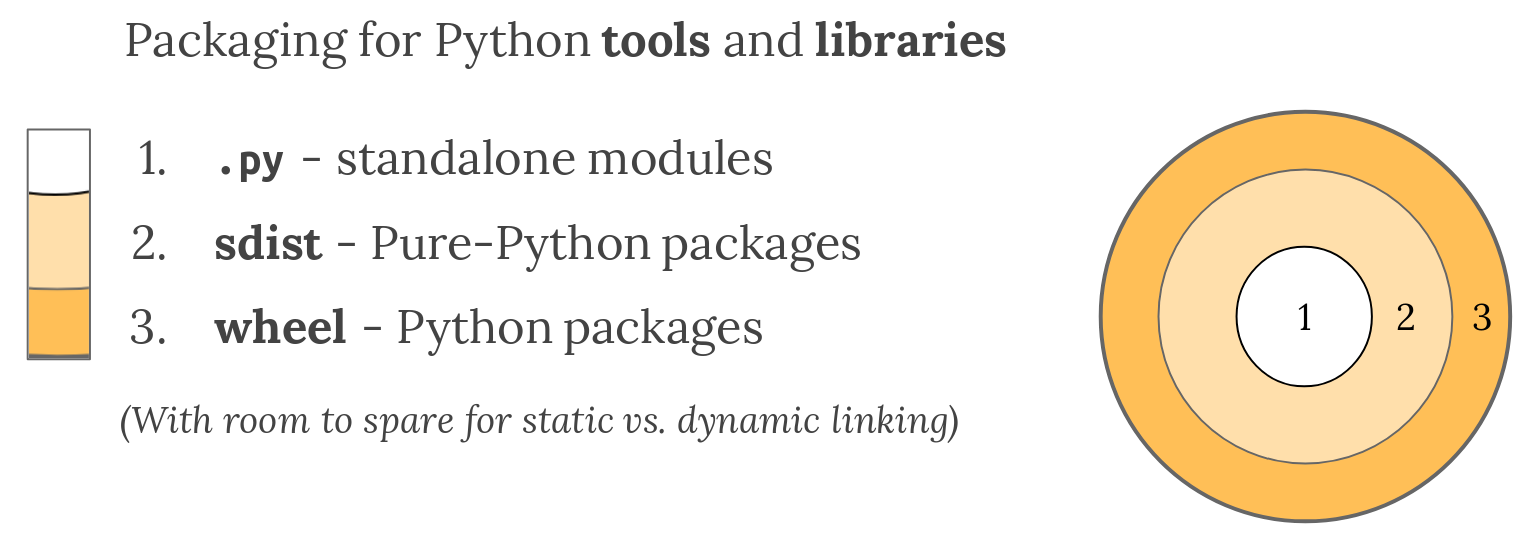
\includegraphics[width=.8\textwidth]{../images/py_pkg_tools_and_libs.png}
\end{figure}

\subsection{打包Python应用}

到现在为止,我们仅仅讨论了Python的原生分发工具。基于我们的介绍,你应该成功地推断出这些自带方法仅仅着眼于有Python并且受众知道如何安装Python包的环境。

随着操作系统、设置和使用者的变化,这样的假设尽在目标是开发者受众时是合理的。

Python的原生打包大部分是为了开发者间分发可复用代码,也就是库创建的。你可以使用例如\text{setuptools entry points}的技术在Python库打包的基础上背驼\textbf{工具}或者针对开发者的基本应用。

库是构建模块,不是完整的应用。对于分发应用,那是一个完全新的世界。

接下来的几个部分根据目标环境的依赖组织应用打包选项,所以你可以选择对于你的项目正确的部分。

\subsection{What about...}

以上部分只能总结如此了,你可能会好奇一些明显的断层。

\subsubsection{操作系统包}

正如前面所提及到的,一些操作系统有它们自己的包管理器。如果你十分了解你的目标操作系统,你可以直接依赖与例如deb或RPM的格式,并且使用那个自建的包管理器来负责安装甚至部署。你甚至可以使用FPM从相同的源生成deb和FPMs。

在大多数部署流水线上,操作系统的包管理器只是帮助你理解的一部分。

\subsubsection{virtualenv}

virtualenvs已经是多代Python开发者不可或缺的工具,但是由于它们被更高层级的工具封装,它们正在退出人们的视野。特别的,对于打包,virtualenvs在the dh-virtualenv tool和osnap中被用作原型,这两个都通过一种自洽的方式封装了virtualenvs。

对于产品部署,不要依赖python -m pip install来将包装入虚拟环境,正如人们可能自开发环境中做得。上面的概述都是更好的解决办法。

\subsubsection{安全性}

你越向下走,更新你的包的组件就越难。所有的东西都联系的越来越紧密。

例如,如果出现了一个内核安全性问题,并且你在部署容器,那么宿主系统的内核可能在不要求构造应用的新代表的情况下更新。如果你不是虚拟机镜像,你将需要一个新的构建。这种动态是否使得某种选择更加安全仍然是一个古老的争论,返回仍未挺停息的问题\href{https://www.google.com/search?channel=fs&q=static+vs+dynamic+linking}{静态vs动态链接}。

\subsection{总结}

Python中的打包由于困难有一定的声望。这种印象大部分是Python的多功能性的副产品。一旦你理解了各种打包策略的自然边界,你开始意识到,变化的景象是Python程序员为了使用最平衡之一的灵活语言的小代价。

\end{document}